\scanpage{27}
% archive foliation: 26
Il y a deux \unsure{choses} à prouver

\uline{Chow raffiné} Si des $F_i$ sont quotients de \unsure{l'un} $\unsure{\simeq}L$, et \unsure{dont} les cycles associés, de \unsure{dimension} $d$, de degré borné, alors, les $F_i$ sont limités
\figure{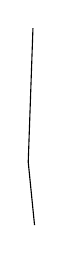
\begin{tikzpicture}\draw (0,0)--(-.06,-1.7)--(.02,-2.5);\end{tikzpicture}}

\deleted{On peut supposer $L=\underline{O}(m)^h$ et par \unsure{$L=\underline{O}^k$}}
En effet, longueur gén. de $F_i$ est à priori bornée, on \unsure{récure} sur le sup. de \deleted{\unsure{ses}}\inserted{ces} longueurs, soit $l$.
Si $l\leq0$, rien à prouver, supposons $\unsure{l\geq1}$.
\deleted{Il \unsure{existe une} \illegible{3}}\inserted{\unsure{pour} $l=1$, alors les} \unsure{énoncés} \unsure{ci-dessus}, \unsure{rien} \deleted{\unsure{à faire}} car \unsure{l'union de|l'un des} \unsure{collections} de faisceaux qui sont limités, \deleted{\unsure{sont}} \unsure{limité|limitée}.
\margin{\textcircled{e}}

Si $l=1$, $F_i\subset\deleted{\unsure{\operatorname{im}}}\underline{O}_{Z_i}$, $Z_i$ un cycle de \deleted{degré} irréductible de degré \deleted{\unsure{\text{cst.}}}\inserted{borné}. Si \deleted{les \unsure{résu}} \deleted{On} \unsure{a} prouvé que les $\underline{O}_{Z_i}$ sont limités, \unsure{il en sera} fini (les uns \unsure{images} d'hom. \unsure{variables} du faisceau $L$ dans $\underline{O}_{Z_i}$). $\unsure{\iota}$
\margin{\textcircled{d}}

Or pour ce dernier fait, on utilise Chow grossier,
\margin{\textcircled{f}}
